\documentclass[10pt,a4paper]{article}
\usepackage[latin1]{inputenc}
\usepackage{amsmath}
\usepackage{amsfonts}
\usepackage{amssymb}
\usepackage{enumitem}
\usepackage{graphicx}
\usepackage{mathtools}
\usepackage[numbers]{natbib}


%opening
\title{Evolution of metabolic networks}
\author{Balint Borgulya}

\begin{document}
	
	
	
	\maketitle
	
	\begin{abstract}
		
	\end{abstract}
	
	\section{TODO}
	\label{sec:todo}
	
	Multiple sources
	Multiple sinks

	Different goal (biomass production also) ON IT'S WAY

	Horizontal gene transfer


	6 carbon CHOPN

	Definitions in footnotes?

	\section{Introduction}

	All life on Earth is based on carbon, and it is hypothesized that if we ever find life on other planets, it will also be based on carbon. CITATION. Carbon can bond with other carbon atoms and different atoms (especially hydrogen, oxygen and nitrogen) to build complex organic molecules. Cells use such complex organic molecules for a variety of functions eg. building their membranes, enzymes and their whole BODY is built using these molecules as building blocks. Cells therefore require organic and inorganic molecules that provide energy, and atoms necessary to synthesise their cellular building blocks.

	The network of chemical reactions responsible for these processes is called the metabolic network (MN) of the cell. MN-s consist of multiple metabolic pathways, that perform a certain function(s) that the organism requires. An example of a metabolic pathway is glycolysis that is the pathway processing glucose (as highly energetic organic compounds) into molecular building blocks (eg. pyruvate) and energy stored in the cell's currency METABOLITE (DEFINE) adenosine triphosphate (ATP).
	
	Chemically speaking it is easy to see that cells have  infinitely many possible ways of metabolising their nutrients to the product they need, if we only impose the constraint that the individual atoms have to be conserved on both sides of reactions.   
	
	Although different organisms utilize different chemical reactions in their MN-s, their core pathways are very similar among many different organisms. Certain pathways are conserved partially  eg. in the glycolytic pathway the Embden-Meyerhof-Parnas (EMP) pathway \cite{EMPpathway} is used by most modern cells for the upper part (also known as the pay-off phase explained in LATER SECTION),  some prokaryotes  use the Entner-Doudoroff (ED) pathway \cite{EDpathway}, while the trunk of the glycolytic pathway is highly conserved. Other pathways such as the citric acid cycle (also known as the Krebs cycle) is used by all aerobic organisms (organisms that live in the presence of oxygen). MAYBE 1 MORE EX

	The reason for these similarities is not yet known, however most authors agree that it is a result of the evolution of the MN-s. 
	Biological evolution is an optimization method, that uses random mutations and the survival of the fittest individuals to evolve organisms to better suit their environments. 



	In this project we will examine whether the high degree of conservedness (CONSERVATIVITY?) of MN-s is an inherent feature of their evolution. To do so we will evolve populations of metabolic networks using an algorithm resembling biological evolution with restricting the networks to simplified yet realistic subset of organic molecules and a toy model of chemistry. We will EXAMINE the reproducibility of evolution, i.e. whether the same MN-s emerge if the "TAPE OF LIFE" is played again. 

	In the following sections we will explain how MN-s can be modelled mathematically as graphs, and how biological evolution can be simulated on a computer, and why this project is of interest to a physicist.

	In the Methods chapter we  will show the methods used in the simulation with emphasis on the subset of molecules used, the calculation of the free energy change, the implementation of evolution in the code, the fitness-comparison of our organisms, and the data analysis. 

	In the Results chapter we summarize the results of the project, giving an example for the fitness calculation, show the results of the population simulations ETC



	
	\subsection{Metabolic networks as graphs}
	Thorough mathematical investigation of these networks reveal interesting topological properties, that make them similar to eg. the social network of humans or the internet. These are small world character, scale-freeness, error-tolerance \cite{largescale} and modularity .
	
	A small-world network \cite{smallworld} is one in which the number of steps to connect any given pair of nodes (in our case chemical compounds) is small, and this number stays constant even as the network grows. In case of the human social networks this is colloquially known as the six degrees of separation \cite{sixdegrees}.
	 
	In a scale-free network the connectivity (the probability that a uniformly chosen node is connected to $n$ other nodes) is $P(n)=n^{-\gamma}$ for some constant $\gamma$, resulting in a few highly connected nodes (Hubs) and many scarcely connected nodes. This provides error-tolerance against random errors to the network, as unless a hub is removed, the performance doesn't decrease significantly. It also makes the network different from a random graph \cite{randomgraphs}, where every node is connected with a constant probability $p$, resulting in a Poisson distribution for the connectivity ($P(k) \approx \frac{\lambda^k e^{-\lambda}}{k!} $), as well as from a regular lattice, where every node is connected to a constant number of other nodes.
	  
	Modules are "by definition, a discrete entity whose function is separable from those of other modules" \cite{modulardef}. Within a module, generally there are multiple possible pathways to achieve the same goal using so called precursor molecules. The module first converts it's input to precursors, and then these are converted to the final product of the module. Usually the module also has the capability to transform precursors to other precursors, providing redundancy to the pathways. Precursors are useful, as if the module lacks one of it's inputs, it is possible that through the conversion of other precursors it can still be functional (even if it functions at a reduced efficiency). Precursors also help evolution, and adaptation, as if the module can use one type of input and process it to precursors, a similar molecule can also be easily converted to the same precursor using perhaps a few additional reactions. Eg. if the cell is capable of processing glucose, using the same enzymatic pathways it is also capable of processing 40 other similar molecules \cite{latent}.
	
	
	
	\subsection{Evolution}\label{chap:evolution}
	
	Evolution works by exploiting the copying errors made when cells divide. After such a division the resulting cell may performance might differ slightly from that of it's predecessor at a certain task. If this change is positive in the sense that it allows the cell to multilply faster it can outcompete the original cell, meaning that in subsequent generations it can overtake the population. (NO TALK OF POPULATION BEFORE) As Charles Darwin wrote "...Natural selection acts only by taking advantage of slight successive variations; she can never take a great and sudden leap, but must advance by short and sure, though slow steps." \cite{darwin} 
	
	It is difficult to imagine how highly sophisticated functions (such as the eye, or feathers for flight, or even a complex metabolic network) could have evolved using slight variations. \cite{latent} argue that complex structures have evolved non-adaptively as exaptations, as byproducts of evolution of other functions. \cite{complexfeatures}  consider simple digital organisms that can obtain energy by performing logic functions. The organisms are provided an environment where they can reproduce (depending on the energy available to them) and mutate, and the more complex logical function they perform, the more energy they receive. They find that although to get to the most complex logical operation (yielding the most amount of energy) many mutations are needed, and when appearing it often destroys other less complex logical operations, once it is present, it provides such value that offsprings that don't have it are quickly eliminated by the competition.
	

	All livingi organisms (except for VIRUSES) code their genetic material in the form of the double helix of DNA (ACRONYM). This uses 3 different base pairs to describe the genetic information of the organism. When the organism multiplies (either sexually or asexually) this information must be doubled and passed on to the offsprings. Even though a multitude of error correcting mechanisms are in place (CITE) errors are made (MAGNITUDE OF ERRORS). These errors are most often point mutations (causing a small change in the genetic code of the organism, in our model  corresponding to adding or removing a reaction from the MN of the cell), and in some cases gene duplications. They are often DELETERIOUS of nature, meaning the offspring will be unfit for life (or at least less fit than the predecessor). 

	Apart from random point mutations  and gene duplications the genetic information of certain cells can also change by the process of horizontal gene transfer.

	Gene duplication is a specific type of error made when copying the genetic material of the cell, resulting in a part of the genetic material to appear twice in the copy \cite{geneduplication}. This is the main source of new genetic material in eukaryotes \cite{horizontalgenetransfer}. Gene duplication is particularly important in light of the modularity of the networks. The robustness of the modules can originate from gene duplication, when a function inside a module is duplicated, and later one copy is evolved to fulfil the function slightly differently. Even if one copy is changed, deleted or (perhaps only temporarily) dysfunctional due to a point mutation the other copy can compensate for this \cite{duplicaterole} \cite{complexfeatures}. 
	
	Horizontal gene transfer is a method allowing Bacteria and Archaea to exchange genetic material between cells. This is thought to be the main reason why bacteria can "learn" from each other eg. resistance to antibiotics \cite{horizontalAntibiotics}\cite{horizontalgenetransfer}.
	
	
	
	\subsection{Artificial chemistries}
	\label{sub:artificial_chemistries}


	When modelling metabolic networks one often has to make simplifications both in theoretical and computational research. These simplifications occur in defining the chemistry the cells can use, the goal function of cells, the environment the cells live in, as well as the anatomy of the cells themselves. SIMPLIFICATION SECTION IN METHODS? GOALS IN SIMULATION, CHEMISTRY BELOW, CELLS BELOW
	
	Modelling the intricacies of chemistry is a hopeless task with today's computers, the fully quantum mechanical treatment of even a few hundred atoms is beyond the capabilities of supercomputers. To overcome this barrier artificial chemistries are often used, that simplify the rules, but grasp some important detail of them. \citeauthor{artificialreview} describes some of these methods used. \citeauthor{evolutioncomplex} use linear molecules consisting of 3 possible  artificial atoms (called "1", "2", and "3" with the numbers showing how many bonds an atom can make with other atoms) to construct a metabolic network of organisms, and examine how they evolve. \citeauthor{computationalframework} considers "chemical reactions as graph rewriting operations, and uses a toy-version of quantum chemistry to derive thermodynamic parameters". MORE ON PREVIOUSLY USED METHODS HERE
	
	NEED MORE OF IT OR MERGE WITH AN OTHER SEC

	
	\subsection{Where is the physics?}\label{chap:whereisphysics}

	In the future - quantum mechanical calculation of the free energy changes of reactions is feasible - better answers then to the same questions

	Stochastic processes when modelling the evolution - Moran process  (it is a reversible Markov chain) - which distribution it draws from - partition functions, random walks on the fittness landscape - stochastic optimization. 
	
	The thermodynamic constraints on evolution - could change temeperature and concentrations. 

	
	
	When calculating the direction of reactions we consider the free-energy change of the substrates and the proucts only. This does not take into account the free energy landscape of the reactions. It would be possible to use quantum mechanics to exactly calculate the free energy change of the reactions used, but it would be a job worthy of it's own project, and therefore we restrict our discussion to estimates of the free energy.
	
	The selection process used when chosing cells to reproduce is the Moran process, a well known Markov chain \cite[]{absorptionofmoran} STOCHASTIC LEARNING PROCESS
	
	EXPAND HERE OR IN METHODS


	
\section{Methods}
\label{sec:methods}

\subsection{The data provided}
\label{sub:What was I provided with?}
List of reactants and reactions, with standard free E changes. 



A set of compounds and reactions (as used by \cite[]{BartekLower}) was provided for the project. The list of compounds consised of 1966 CHOPN molecules of at most 3 carbon atoms, along with 13 so called internal metabolites (compounds that are not necessariliy CHOPN molecules fitting the previous criteria, but they are essential to the reactions in the MN-s, listed in Table \ref{environmentTable}). Internal metabolites are considered to be present in the cell, with the concentration as mentioned in Table \ref{environmentTable}. Later I intend to test the networks using different concentrations.(DO I?). We assume a steady INFLUX of the starting compound is available, and a steady flux of the end product (eg. pyruvate ) is removed (used by the cell), and every other metabolite has to be created and used by the MN.. 
	
	There are 11790 reactions of the at most 3 carbon compounds in the database used along with the reactants, the products and the free energy change of the reaction at standard conditions. The free energy changes are later calculated for arbitrary conditions as discussed in Section \ref{sub:The free energy change}
	
\subsubsection{Restrictions on chemistry}
\label{ssub:Restrictions on chemistry}
What compounds are used, why?
Previous author's restrictions on artificial chemistries. Should this go to Intro? yes they should 

	We will restrict the reactions available to the organisms we simulate to those using CHOPN molecules (containing only carbon, hydrogen, oxygen, phosphor and nitrogen) of at most 3 carbon atoms initially, with later increasing the maximal number of carbon atoms to $6$ . This is a realistic constraint as the TRUNK PICTURE? of the glycolytic pathway consists of such molecules considered initialy. The initial list of the molecules and reactions used are the same used by \cite{BartekLower}, and were provided by the project supervisor as described in Section \ref{sub:What was I provided with?}. The extended set of molecules and reactions were also generated and supplied by the project supervisor, with the methods of generation described in \cite[]{BartekLower}.

	An other assumption made in our model is that the direction of a reaction is determined only by it's free energy change as defined under the circumstances of the simulation. It is also assumed that given two reactions, both with free energy change larger (or smaller) than some pre-defined limit $L$ the maximal FLUX (number of reactions happening per unit time on an arbitrary scale)) (DEFINE) through both reactions is the same. This is not necessarily the case in real cells, and in addition to the free energy difference, the speed and direction of the reaction can be influenced by the free energy landscape between the initial and final states and by the cell via the use of enzymes. 

	The constraints imposed on the flux of each reaction, depending on the free energy change of them are as follows: for the $m$th reaction the flux $v_m$ has to satisfy $0\leq v_m \leq 1 $ if $\Delta G \leq -L$~eV, $-1\leq v_m \leq 0 $ if $\Delta G \geq L$~eV. As in the real world the reactions happening in a cell are usually reversible with (an example for this is is the reaction of carbonic acid and water H$_2$CO$_3$$_{(l)}$ + H$_2$O$_{(l)} \leftrightarrows$ HCO$^-_3$$_{(aq)}$+H$_3$O$^+$$_{(aq)}$), we allow reactions with free energy change between a constant $-L$ and $L$ eV to happen in any direction. Currently the value of $L=10$~eV but it is a parameter easily changed in the program. 

	
	
	\subsection{Anatomy of the oganisms simulated}
	\label{ssub:anatomy_of_the_oganisms_simulated}
	
	The anatomy of our cells is as follows: the cells are stationary with certain compounds present within their body with concentrations as shown in Table \ref{environmentTable}. The cells can import and export $H_2$O and CO$_2$ to and from their environments to replenish their reserves, if these compounds are used by their MN. They can also import one (planning to include more) predefined nutrient to process, and they can dispose  one (planning to allow more) target molecule (NOTE: this molecule is only disposed from the viewpoint of the metabolic pathway. It is often further processed by subsequent pathways, with the example of pyruvate, that is the end product of the UPPER PART of glycolysis, which is later fed into the citric acid cycle). In real life a certain allele (DEFINE) can spread in the population if it provides an reproductive advantage to the cells carrying it.  As ATP acts as the energy currency in cells (they can hydrolise ATP into ADP in a HIGHLY? exotermic reaction) the fittness (DEFINE) measured by the cell's ADP $\rightarrow$ATP conversion rate is proportional to the growth rate of the cells, as reproduction (or division) is a very energy-demanding (AND BIOMASS?) process for the cells.  The implementation of more complex goal functions along with multiple input and output molecules is planned, eg. biomass production, which is also a requirement for reproduction. 

	DO WE NEED STATIONARITY?

	Each of our cells has chance to reproduce, and this chance is proportional to their current fitness value, ensuring that cells with negative fittness (considered ELETKEPTELEN?).  The selection of cells ACCORDING TO this probability density function is done using the Moran process, described in Section \ref{sub:Implementing evolution}

	We consider a constant sized population (which is reasonable in a space/FOOD DEPRIVED environment), meaning that every time a cell reproduces, a cell must die to accomodate the newborn one. The decasing cell is chosen uniformly from the population, therefore giving the expected lifetime of a cell to be 1 GENERATION (DEFINE). Constant life expectency is OBSERVED? in nature, and along with the fitness-weighted selection for reproduction results in more expected reproductions for fitter organisms. 

	The cells in a population are considered to be close to each other, so  any two cells can meet and exchange genetic information in the process of horizontal gene transfer (IF IMPLEMENTED) (when reproducing any cell can take over any other cell. (CELLS DYING BEING REPLACED). Also)


\subsection{Calculating the free energy change}
\label{sub:The free energy change}
The physics of the formula to calculate it. The role of deciding the direction of reactions.  $\rightarrow$ valid ranges  that can be changed at the beginning of the program.



	The list of reactions provided to me by my supervisor contained the following for each reaction: 
	\begin{enumerate}
		\item List of compounds the reaction uses
		\item List of product the reaction produces
		\item The free energy change of the reaction (experimentally when known, otherwise estimated) \cite{BartekLower}
	\end{enumerate}
	
	The free energy changes provided were at standard conditions $T=25  ^o C$ pH$=7.0$ $I=0.2 M$ (ionic strength) and all metabolite concentrations set to 1~M.
	
	Assuming a reaction of the form $n_1A + n_2B \leftrightarrows n_3C + n_4D$ where the concentration of substrate $A$ is denoted by $[A]$, and similarly for the other substrates. $n_1$ denotes the number of molecules of type $A$ that take part in the reaction and  $\Delta G^0$  the free energy change of this reaction at standard conditions. The change in free energy for arbitrary $T$ and concentrations is given by: 
	
	\begin{equation}\label{eq:freeechange}
		\Delta G = \Delta G^0 + R T \ln \frac{[C]^{n_3}[D]^{n_4}}{[A]^{n_1}[B]^{n_2}}
	\end{equation}
	
	At the beginning of the program the reactions are read in from a file, and the free energy changes are re-calculated for the specified conditions as in Table \ref{environmentTable}. UPDATE
	
	\begin{table}
		\centering
	\begin{tabular}{|c|c|}
		
		\hline Temperature & 293 K \\ 
		\hline [ATP] & $10^{-1} M$ \\ 
		\hline [ADP] & $10^{-2} M$ \\ 
		\hline [AMP] & $10^{-4} M$ \\ 
		\hline [NAD] & $10^{-2} M$ \\ 
		\hline [NADH] & $10^{-2} M$ \\ 
		\hline [Pi] &  $10^{-3} M$\\ 
		\hline [PPi] & $10^{-3} M$ \\ 
		\hline [CO$_2$] & $10^{-5} M$ \\ 
		\hline [NH$_3$] & $10^{-5} M$ \\ 

		\hline 
	\end{tabular} 
	\caption{The environmental variables currently PUT THE OTHER ONES IN TOO}
	\label{environmentTable}
	\end{table}





\subsection{In silico Evolution}
\label{sub:Implementing evolution}

Do not break up into subsections

The possible mutations, why it makes sense to use only these, and possible other mutations that could have been used. The rate of mutations. 

INTRO SENTENCE

	The real evolution of the genomes of organisms uses a variety of methods as discussed in Section \ref{chap:evolution}. Of these, my cells use point mutations, that either add or delete a reaction that is currently available to them. Simply adding a reaction to those available to the cell at random from the list of all the reactions is unlikely to result in a reaction that would be used by the cell, as with a high probability the added reaction would use reactants that are not present in the cell (the added reaction would be disconnected from the current MN), and produce compounds that are not used in it. As discussed in Section \ref{sub:Flux Balance analysis} the flux through these reactions would be zero. Therefore when adding reactions, I only consider those that are linked  to one of the current reactions, either by using a compound that  the network is capable of producing, or providing one that it can consume. EXAMPLE FOR TRIAL NETWORK USED IN FBA SECTION? This way the graph of the reactions and compounds available to the cell stays a connected graph (disregarding deletions). Choosing the list of reactions that can be added uses the neighbour-list defined in Section \ref{sub:Storing the reaction network}. When deleting a reaction every currently available reaction has equal probability of being deleted. This can and does result in DISCONNECTED graphs, but such disconnected parts are usually small, otherwise they bear too high a cost to maintain (COSt OF REACTIONS).  
	
	\subsubsection{Reproduction TO BE DELETED}
\label{ssub:Reproduction}
survival of the fittest using the Moran process - Metropolis algorithm?
Moran process - reversible markov chain
Detailed balance equation

\subsubsection{Competition TO BE DELETED}
\label{ssub:Competition}
Goal functions? $\rightarrow$ changing goal functions? Talk about trial networks (ethanol producing)?

The probability density function (PDF) of which cell is selected for reproduction is proportional to the fitness of each cell (with the CAVEAT that cells with negative fitness are deemed unviable and are not allowed to reproduce). To know this PDF it is necessary to know the fitness of each cell at any given time point, and therefore it would be impractical to use this to chose the cell that will reproduce. Instead we use the Moran process \cite{moranprocess}, a well known reversible Markov chain originally used to calculate the time a mutation takes to spread in a population. This process works as follows: (LIST?) first we uniformly chose a cell in our population. Then we generate a random number from the distribution $U \left( r,M \right)$ where $M$ is the maximal fitness value a cell can take. Let us denote the fitness of the chosen cell by $F_c$. Then if $F_c \geq r$ we accept the change, if not we start the process again. 

This process CAN BE SHOWN to result in a sampling of cells equivalent to that of the PDF proportional to the fitness of each cell. DETAILED BALANCE ~ GIBBS etc

\subsection{Flux Balance analysis}
\label{sub:Flux Balance analysis}

Detailed description $\rightarrow$ equations, example matrix? Which fluxes are free? Which fluxes are limited? GLPK 



	To calculate the throughput of the metabolic network of my organisms I use flux balance analysis \cite{whatisfluxbalance}. This method is computationally fast and easy to implement, however it disregards most of the thermodynamic and chemical constraints on the speed of the reactions. By using it I make the assumption that all reactions happen at equal speeds, given the reactants are present the reaction will happen, and the direction of a reaction is defined by the free energy change at the specific conditions. It doesn't take into account the free energy landscape of the reaction, whether an energy barrier is blocking the reaction etc. (partially duplicate from section \ref{chap:whereisphysics}). The disregard of the energy barriers is justified by considering the cell's ability to lower such barriers using catalyst enzymes.
	
	The goal of flux balance analysis is to calculate the steady state fluxes ($\mathbf{v}$) through all the reactions subject to some constraints, (described later in this section), while maximizing a function $Z=\mathbf{c}^T \mathbf{v}$ of the fluxes in the solution space allowed by the constraints. 

	\begin{figure}[t]
		\centering
		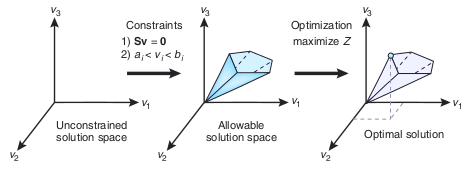
\includegraphics[width=0.8\linewidth]{fba_frompaper.png}
		\caption{The process of flux balance analysis. First we apply the steady state constraints along with FURTHER CONSTRAINTS on the fluxes, then we maximize the goal function in the allowable solution space found. Figure from \cite[]{whatisfluxbalance} }
		\label{fig:fluxbalance}
	\end{figure}

	When using flux balance analysis we represent the MB as a stoichiometric matrix $S$ ($m\times n$), with each row corresponding to a compound in the network ($n$ compounds), and each column corresponding to a reaction ($m$ reactions). In each column we have the stoichiometric coefficients of the given reaction that correspond to the compound of the given row. Negative stoichiometric coefficients are used for the metabolites consumed, positive for those produced, and zeros for the metabolites that do not participate in the given reaction.
 
	The steady state assumption of the method means that the amount of any given compound produced in the reactions should equal the amount consumed by other reactions, except for some special compounds. These compounds are considered the nutrients and the end-products of a metabolic network. For example the nutrients of our network is FIRST COMPOUND, water and $O_2$, while it's end products are pyruvate and $CO_2$. To incorporate compounds that can have a non-zero change in CONCENTRATION could be introduced to flux balance analysis could be done through relaxing the constraint that the EQUATION-s of these compounds have to equal zero. This introduces complications, as often the amount of certain compounds produced appear in the goal function  $Z=\mathbf{c}^T \mathbf{v}$. To overcome this we introduce auxiliary reactions to the stoichiometric matrix $S$, for the compounds the cell consumes and produces. Such an auxiliary reaction is for example $ \rightarrow H_2O$, that "creates water out of nothing", or in other words corresponds to the potential water intake of the cell ENABLING THE CELL TO TAKE UP WATER?

	As the fluxes are calculated on an arbitrary scale, we can impose an arbitrary bound on the fluxes of real (non-auxiliary) reactions.


	The form of the goal function is $Z=\mathbf{c}^T \mathbf{v}$ with the elements of $\mathbf{c}$ being the weights of the fluxes through each reaction in the goal function. In the simplest cases $c_i=0$ for all but a single value of $i$, in this case the goal is to maximize the flux through a single reaction, which is often chosen to be the biomass removing auxiliary equation. In our case the goal function used is the one converting ATP to ADP. This reaction occurs in cells, (ATP~+H$_2$O~$\rightarrow$~ADP~+~P$_i$), and it is a highly exothermic reaction. Cells store energy in ATP molecules, and release this energy by converting them into ADP, therefore by maximizing the flux through this reaction, we are maximizing the energy output of the cell. In many cases this is synonymous with maximizing the growth rate of the cell. (CITATION). OTHER GOAL FUNCTIONS?
	
	There are many software packages capable of solving linear programming problems, we use the Gnu Linear Programming Kit (GLPK) \cite{glpk}. GLPK is implemented in C, and has all the functionality we need to calculate the fitness of our metabolic network. For the code calculating the fitnesses see calcThroughput in APPENDIX.


	OLD FROM HERE TILL NEXT CHAPTER

	
	Flux balance analysis works by trying to find the fluxes through the set of reactions available to the cell that maximize a certain goal function. This is done while keeping the fluxes such that they represent a steady state solution to the reaction network, meaning that any product created is used by an other reaction, and any reactants used are produced by an other reaction, except for the source and sink substrate and some internal metabolites. This is a reasonable assumption as cells usually import a small set of molecules (the source substrates, water, O$_2$, etc.) and use them up to build their own matter while disposing of again a few substrates (eg. CO$_2$). Throughout the flux balance analysis it is assumed that a large (but finite) amount of water is available for the cell to use, along with a smaller amount of the source substrate, and the cell can dispose of a large (but finite) amount of CO$_2$, along with a smaller amount of the sink substrate. Disposing of the sink substrate in this context means that it leaves the metabolic network, but not necessarily the cell, as it is often used to build the cell itself, or further processed by other metabolic networks (eg. pyruvate).
	
	The mathematical execution of flux balance analysis is essentially a linear programming problem. In my program I solve this using the Gnu Linear Programming Kit (GLPK) \cite{glpk}. GLPK needs to be provided the stoichiometric matrix (MORE ABOUT THIS MATRIX? EXAMPLE?) with $n$ columns and $m$ rows, where $n$ is the number of reactions currently in the network, and $m$ is the number of substrates the reaction uses.  
	
	To enable the addition and removal of substrates to and from the cell auxiliary reactions are added to the ones available to the cell. These reactions do not appear in the cell and are not valid chemical reactions, they are simply expressing a flux to or from the cell. (eg. there is an auxiliary reaction that creates H$_2$O out of nothing) There are auxiliary reactions creating H$_2$O, the source substrate, and there are ones removing CO$_2$ and the sink substrate. There is also one that corresponds to a real reaction, the hydrolysis of ATP to ADP cells use to free up and use the energy stored by glycolysis (ATP~+H$_2$O~$\rightarrow$~ADP~+~P$_i$). In the glycolysis simulation the goal function was the flux of this previous reaction. 
	TALK ABOUT OTHER GOAL FUNCTIONS HERE?
\subsection{Data analysis}
\label{sub:visualization}

the use of Cytoscape $\rightarrow$ xgmml format and the  program part to output that

\subsection{Population simulation}
\label{sub:population_simulation}
How to store the population, how to choose which one to mutate (as in \ref{ssub:Reproduction}. 

New method of storing indexes only. Include the previous method too?



\subsection{Comparing populations}
\label{sub:comparing_populations}


\subsubsection{Similarity Index}
\label{ssub:Similarity Index}

How to calculate, why is it useful? Can be calculated for nonzero flux reactions or all available ones too. 

\subsubsection{Inverse participation ratio}
\label{ssub:Inverse participation ratio}
IPR vs Entropy

\subsection{Technical bits RENAME}
\label{sub:technical_bits_rename}

\subsection{Random number generation}
\label{sub:Random number generation}

Good quality random numbers $\rightarrow$ mt19937 Mersenne Twister. Reproducibility is important $\rightarrow$ seeds always known. 

As one of the main components of the process of evolution is the random mutations when cells divide, we will need to use random numbers in the program. Generating true random numbers is a cumbersome process, that uses an inherently random physical process (eg. thermal or atmospheric noise, radioactive decay counts, or quantum phenomena \cite{truerandom}) to produce random numbers. For most applications however it suffices to use Pseudo Random Number Generators (PRNG-s) to generate numbers that appear random, in a sense that they pass certain tests of randomness \cite[]{randomtests}. These PRNG-s use an initial value called seed (or multiple initial values), the knowledge of which allows anyone to calculate any element of the series of pseudorandom numbers. In applications where there is need for the unpredictability of the series (eg. cryptography) the seed(s) is chosen using a process that is considered to be random (eg. the time held by the computer's clock in nanoseconds, or the movement of the mouse under a sufficiently long time).

In our case there is no need for such unpredictability, on the contrary, we would like the evolutions of populations to be reproducible (either by ourselves, for error checking, or by other researchers), however we would like to simulate multiple populations of cells with different underlying random numbers (to be independent from each other). This is easy to achieve, by using consecutive integers as seeds for the different parallel runs, and noting these numbers in the files produced by the program. This way if we start two populations using the same seed (and the same initial conditions) the results of the two simulations will be identical. 

PRNG-s generate use the seeds to initialize their internal state, which is a set of bits the generator uses and changes whenever it produces a new pseudorandom number. As the internal state consists of a finite number of bits, given enough pseudorandom numbers are requested from the generator, the outputs will start to repeat themselves. The number of pseudorandom numbers we can get from a PRNG without repetition is called it's period. The default PRNG in C++ (\texttt{rand()}) has a period of $2^{32}$. As we would like to simulate the populations of cells for more than $2^{32}$ reproductions, we use the Mersenne Twister \cite{mersennetwister} generator, provided by the Boost C++ Libraries \cite{boostlibraries}. This generator is fast, provides high-quality pseudorandom numbers and has a period of $2^{19937}-1$, and will therefore provide more than enough random numbers for our simulations. In addition the Boost implementation is capable of producing both integers, and reals on given intervals. 


\subsection{Storing the reaction network}
\label{sub:Storing the reaction network}
Structure of the input files -$\rightarrow$ algorithm to read them in $\rightarrow$ store them. 

The neighbour list and it's use in adding reactions.



	After they are read in from a file substrates are stored in a substrate object that store the index of the molecule, the free energy of creation, the name, the chemical formula, the charge, and a list of reactions it is involved in. This list is generated when reading in the reactions from the file provided.
	
	Reactions are stored in reaction objects that store the index, the substrates  (starting compounds), the products  (final compounds), the free energy change at standard conditions, the free energy change at the current conditions (calculated later), and the neighbouring reactions (calculated later) of the reaction. The free energy change of reactions is recalculated at the beginning of each run as described in Section \ref{sub:The free energy change}
	
	The original idea was to store the reaction network as a Graph object provided by the Boost Graph Library \cite{boostlibraries}. This was a feature rich graph implementation that allowed searching for neighbouring reactions that can be added (EXPLAINED LATER), however as it uses sophisticated methods (TALK ABOUT TEMPLATES?) to store the  graphs and therefore for the evolution of a single organism it could only calculate approximately 2 generations per second. 
	
	To speed up the calculations simple vectors were used to store the compound and reaction objects, such that each compound object contained a list of the reactions it appears in. Using this at the beginning of the program a neighbour-list was generated that for every reaction contained a list of neighbouring reactions, that share at least 1 compound with it (excluding internal metabolites). (EXAMPLE?) Using this neighbour-list the program was now able to handle $\sim 100$ generations per second. 

\subsubsection{Parallel simulations}
\label{ssub:Paralell simulations}
Multiple populations with same initial network  run parallel$\rightarrow$ different random seed. Cplab machines, talk about the distributing/collecting scripts?



\section{Results}
\label{sec:results}


\subsection{Example of flux balance analysis}
\label{sub:example_of_flux_balance_analysis}


	As an example for such a stoichiometric matrix we show that of a simple network that was used for testing the part of the algorithm that executes flux balance analysis. Let us consider the metabolic network shown on Figure \ref{fig:examplenetwork}. The metabolites (in green) have been denoted by letters A, B and D. MAKE CO2 RED!!! The stoichiometric matrix of this metabolic network is shown at Equation~\ref{eq:examplematrix} (below). The metabolites each row corresponds to are shown on the LHS of the matrix. The first three columns of the matrix correspond to reactions $5151$, $5133$ and $131$ respectively. The other columns correspond to auxiliary reactions, providing the nutrient of the network (A), removing the end-product (lactate), providing water, providing CO$_2$, and converting ATP to ADP. 

\begin{figure}[t]
	\centering
	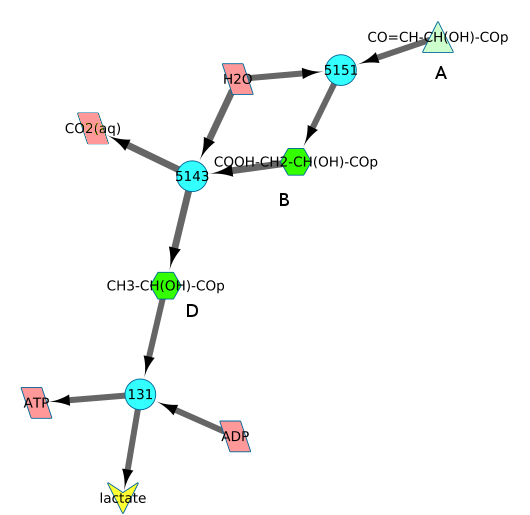
\includegraphics[width=0.5\linewidth]{initial_network_ABC.png}
	\caption{Example of a simple network. Reactions: light blue, metabolites: green, nutrient: light green, end-product: yellow, internal metabolites:red}
	\label{fig:examplenetwork}
\end{figure}

	\begin{equation}
	\begin{matrix}
		\texttt{A}   \\
		\texttt{B}\\
		\texttt{D}\\
		\texttt{lactate}\\
		\texttt{water}\\
		\texttt{CO}_2\\
		\texttt{ATP}\\
		\texttt{ADP}
	\end{matrix}
	,S=
	\begin{pmatrix}
			%\hline Fluxes: & 1 & 1 & 1 & 1 & 1 & 3 & -3 & \color{red} $\mathbf{1}$ \\
			%\hline	Reaction: & 5151& 5143 & 131 & \multicolumn{4}{c|}{Auxiliary }& Target \\
			  -1 &  0 &  0 & +1 &  0 &  0 & 0 & 0 & \\ 
			  +1 & -1 &  0 &  0 &  0 &  0 & 0 &0 &  \\ 
			  0 & +1 & -1 &  0 &  0 &  0 & 0 & 0 & \\ 
			  0  &  0 & +1 &  0 & -1 &  0 & 0 & 0 & \\ 
			  -1 & -1 &  0 &  0 &  0 &+1  & 0 & 0 & \\ 
			  +1 & +1 &  0 &  0 &  0 &  0 & +1&0 &  \\ 
			  0 & +1 &  0 &  0 &  0 & 0 &0 & -1 &\\ 
			  0 & -1 &  0 &  0 &  0 & 0 &0 & +1 & \\ 
			  
		\end{pmatrix} 
		\label{eq:examplematrix}
	\end{equation}


	Flux balance analysis finds the set of fluxes $\mathbf{v}=\left( v_1,v_2,...,v_m \right)$, that satisfy $S\mathbf{v}=\mathbf{0}$ and maximize the goal function $f \left( \mathbf{v} \right)$. The linear equations that are implied by $S\mathbf{v}=\mathbf{0}$ for the example network of Figure \ref{fig:examplenetwork} are shown below, at Equation \ref{eq:lineqs}. Constraints on the system are imposed in two ways. Firstly by $S\mathbf{v}=0$ we require that the fluxes represent the steady state solution, and secondly by restricting the values of $v_i$ by inequalities ($v_{lower,i}\leq v_i \leq v_{higher,i}$) we can restrict the flux of individual reactions, their directions, and the amount of COMPOUNDS the cell can take up and dispose of. 
	

	\begin{equation}\label{eq:lineqs}
		\begin{matrix}
			- v_1+v_4=0 \\
			v_1-v_2=0 \\
			v_2-v_3=0 \\
			v_3-v_5=0 \\
			-v_1-v_2+v_6=0 \\
			v_1+v_2+v_7=0 \\
			v_2-v_8=0 \\
			-v_2+v_8=0
		\end{matrix}
	\end{equation}



\subsection{Similar networks reached in parallel runs}
\label{sub:similar_networks_reached_in_paralell_runs}


If mutations happen with 100$\%$ then rather fast improvement to best network. Very diverse populations in terms of available reactions, but somewhat similar within a single run. Different runs very different available reactions. For the nonzero flux reactions within a run is almost completely homogeneous, and lots of similarity between runs too. 

If the mutation probabilities decrease improvements become more difficult.

\subsection{Limitations}
\label{sub:limitations}
Dynamics of chemical reactions ignored

Restrictions in the types of mutations

Small interactions between cells

Too simple goal function



\section{Discussion}
\label{sec:discussion}


%	\iffalse
%	
%	\subsection{Simulation not needed}
%	
%	To simulate evolution on a computer we need three things: replication, mutation and competition. Algorithms empowered by the evolutionary principles \cite{evolutionaryalgorithms} are used every day now to find optimal solutions to problems in all fields of science. These algorithms need a function for which to optimize the given system, called the goal function. The goal function of real-world cells is rather complex, with goals reaching from growth to reproduction. Translating these goals to the language of mathematics and computers is not an easy task. \cite{complexfeatures} sets the execution of more complex logical operations as a goal for the digital organisms in question. \cite{evolutioncomplex} use the import of precursors and their procession to more complex molecules as the goal function. 
%	
%	In my simulations I consider the rate of ADP-ATP conversion as the goal function after \cite{BartekLower}, however later I plan to experiment with different goal functions that also consider the amount of carbon products produced (that can be used for building the cell). 
%	
%	\section{trol}
%	The core of the energy producing metabolic pathways of organisms are very similar, for all three domains of life, however there are many pathways that are chemically viable.  The throughput of these pathways greatly influences the fitness of any given organism. 
%	
%	Cells usually convert their input material into precursor molecules, which are then converted into the biomass of the cell and energy. This method is robust in terms of input molecules, as described in \cite{latent} the ability to synthesize all biomass from a single source of carbon and energy enables the cell to use molecules similar to the original. Eg. if the cell is capable of processing glucose, using the same enzymatic pathways it is also capable of processing 40 other similar molecules.  In \cite{latent} the authors examine how an evolutionary advantage can originate from an exaptation. 
%	
%	  
%	Most modern cells use the the Embden-Meyerhof-Parnas (EMP) pathway for the upper part of the glycotic  pathway, while some prokaryotes use the Entner-Doudoroff (ED) pathway \cite{EDpathway}. The trunk of the pathway however is highly conserved and so are the enzymes used \cite{latent}. 
%	
%	The similarity can occur for a variety of reasons, it can be due to the current pathways being the most optimal one given the set of constraints posed by the environment of the cells as described in \cite{theoretical}, \cite{central}. It can also occur because of historical reasons \cite{historical}. In this article the authors examine whether chemically viable metabolic pathways are connected in the sense of being able to mutate (using one-reaction mutations) from one pathway to an other while preserving viability. They find that in all but the simplest metabolisms this is possible.
%	
%	In \cite{theoretical} it is found that the metabolic network of modern cell (the EMP pathway) is optimized to provide the highest possible ATP production flux, while maintaining a high kinetic efficiency. 
%	
%	The central carbon metabolism of the E. coli. bacteria is examined in \cite{central}. This converts sugars into metabolic precursors which are then in turn converted to the biomass of the cell, and energy. The authors try to find a simplifying principle for the structure of the metabolic network, and find that it can be considered as a minimal walk (in terms of enzymatic steps) between any pair of the 12 metabolic precursors for the biomass of the cell, and the one that is responsible for the ATP balance. In addition the enzymatic distance between the precursors and the input sugars is also minimized suggesting that the pathway used is optimal in this sense. 
%	
%	There are exceptions of this similarity, as mentioned in \cite{strategy} the glucose metabolism of procaryotic cells shows a great variety. The canonical pathway used by most organisms is the EMP pathway producing 2 ATP molecules for every glucose consumed, but the alternative Entner-Doudoroff (ED) pathway which only produces 1 ATP per glucose is still viable, as it requires much less enzymatic proteins than the EMP pathway to achieve the same glucose conversion rate. This is thought to present an evolutionary advantage that makes up for the reduced ATP production rate. 
%	
%	\subsection{Computational approach}
%	
%	Apart from the analytic work done in the field, with the increase of processing power simulations became a valuable tool in modelling metabolic networks. Simulations can be exhaustive (looking through all the chemically feasible reaction chains), or simulating evolution. 
%	
%	According to Daniel Dennett "... evolution will occure whenever and wherever three conditions are met: replication, variation (mutation), and differential fitness (competition)". REFERENCE THIS 
%	Simulating the evolution of metabolic networks is a difficult task even for today's computers. To accurately calculate efficiencies in different environments we would have to implement chemistry as a whole. To make the problems more manageable artificial chemistries are considered in some cases \cite{artificialreview} \cite{artificialshort}.
%	
%
%	Charles Darwin having discovered evolution \cite{darwin} realized that the highly  sophisticated organs such as the eye must have evolved through many steps. In \cite{latent} the authors argue that as other complex structures (such as feathers for flight) have evolved non-adaptively as exaptations, as byproducts of evolution of other functions. In \cite{complexfeatures} the authors consider simple digital organisms that can obtain energy by performing logic functions. The organisms are provided an environment where they can reproduce and mutate, and the more complex logical function they perform, the more energy they receive. They find that although to get to the most complex (and most energy yielding) operations many mutations are needed, once it is present, it provides such value that offsprings that don't have it are quickly eliminated by the competition. Supports the claims of \cite{latent}.
%	
%	These metabolic networks shows resemblance to highly error tolerant scale-free networks \cite{largescale} that have some highly connected nodes (compounds) which take part in many reactions. The networks are tolerant to random errors (removal of reactions or molecules). Similar conclusions are drawn in \cite{complexfeatures} which also examines the modularity property of metabolic networks by simulating artificial organisms living on a 2D surface, operating on artificial molecules. They find that gene-pairs that when removed individually do not influence the performance of the organism greatly, but when removed together  they are lethal, occur within strongly interconnected modules. The functions of these modules are separable, this contributes to their error-tolerance. Both of these articles mention the small world \cite{smallworld} property of the networks, meaning that they are "highly clustered, like regular lattices, yet have small characteristic path lengths, like random graphs." This property makes them similar to social networks of humans. 
%	
%	In \cite{computationalframework} the authors "employ an artificial chemistry that views chemical reactions graph rewriting operations and utilizes a toy-version of quantum chemistry to derive thermodynamic parameters." 
%	
%	\fi
	
\section{Sentences that don't fit anywhere}
\label{sec:sentences_that_don_t_fit_anywhere}

This way, depending on the specific needs of the cell the direction of reactions can be reversed, eg. in the case of glycosis (processing sugars to energy and simpler molecules)- glyconeogenesis (producing sugars by using energy and simpler molecules).


	LOWER The reason for these similarities is yet to be discovered, but the two most common hypothesis  are : 
	\begin{enumerate}[label=(\alph*)]
	\item the best possible metabolic network has been found, evolution finished the optimization and there is no possible further improvement (Global maximum found) \cite{theoretical} \cite{latent} \cite{strategy}, or 
	\item there is a better solution but to get there cells have to evolve through such suboptimal states, that are outcompeted by the current metabolic networks. (Local maximum found) FIND SOURCE HERE
	\end{enumerate} 
	 \cite{historical} reasons that (b) is unlikely, as they find that  "most viable metabolisms can be transformed into one another by single viability-preserving reaction changes."  
	
	PICTURE? we can imagine two reactions with equal free energies at the substrates and products, one transitioning smooth from substrate to product, the other having a large energy barrier between. Clearly the one with the barrier would not (or much more rarely) happen in a cell than the smooth transitioning. This is simplification is balanced by the fact that cells can use enzymes to act as catalysts to these reactions lowering such energy barriers. Should they need cells can also raise such barriers to otherwise smoothly transitioning reactions to stop them from occurring. 



	\bibliography{dissertation}
	\bibliographystyle{plainnat}
\end{document}
